% !TeX root = RJwrapper.tex
\title{atime for asymptotic timings }
\author{Doris Amoakohene, Toby Hocking, Anirban Chetia}

\maketitle

\abstract{}
When developing R packages, understanding how your code performs is important. This is why analyzing time complexity is beneficial, and asymptotic timings help us understand how algorithms scale as data size increases, providing performance insights. Previous work has produced various packages and functions for performance benchmarking, yet we often do not prioritize time and memory complexity, even though they are important.
We propose a new package named \code{atime} for asymptotic timing, performance testing, and comparative benchmarking. We are evaluating the features of \code{atime} against previous functions and packages, investigating the GitHub Action that uses it, and comparing its performance with other R packages that utilize GitHub Actions. 

\section{Introduction}
The performance of an R package provides utilities for computing measures to assess model quality, many of which are not directly provided by R's \texttt{base} or \texttt{stats} packages as discussed by \cite{system.time}. In the field of computer science and algorithm development, performance analysis plays a crucial role in determining the efficiency and effectiveness of different algorithms as mentioned in \cite{knuth1997art}. Performance analysis helps us identify the most efficient algorithms for a given task, optimize code versions, and make informed decisions about algorithm selection in real-world applications. Several factors contributing to an algorithm's performance, including its time and memory complexity, are discussed in the latest edition of introdution to algorithms \cite{cormen2022introduction}.\\

\noindent Understanding the \code{atime} package requires knowledge of asymptotic complexity, also known as "Big O" notation. Asymptotic complexity describes how an algorithm's runtime or memory usage scales as the size of the input data increases. Analyzing performance characteristics, including time and space complexity, is critical when working with large datasets. In \cite{Hocking2021}, his analysis provides valuable insights into trade-offs between convenience and computational efficiency, enabling users to make informed decisions when selecting data reshaping tools.
 
\noindent \cite{suh2017emp} discusses the importance of accurately measuring a program execution time, a common performance evaluation technique in computer science research. They highlight the distinction between elapsed time (ET) and process time (PT), where ET represents the end-to-end time of a program, while PT focuses solely on the execution time of the process of interest. \texttt{atime} addresses this challenge by providing a powerful tool for analyzing and comparing the asymptotic time and memory usage of different R programs.

\noindent Several packages such as \texttt{microbenchmark} by \cite{microbenchmark}, \texttt{bench} by \cite{bench}, and \texttt{system.time} by \cite{system.time} exist for benchmarking asymptotic timings. This section discusses these packages and compares them with \texttt{atime}. Unlike the functions from these packages which compare timings for a single value, \texttt{atime} allows users to check execution time over a sequence of data sizes (\texttt{N}) and visualize the results.
\\ 
 
\noindent The \texttt{atime} package is designed to analyze algorithm asymptotic time complexity. It provides a simple and efficient way to measure code performance, enabling users to understand how it scales with increasing input size. \code{atime()} works by repeatedly executing a function or algorithm with varying input sizes and measuring the time taken to complete each run. \\

\noindent This article provides an overview and description of the package and its applications, explaining its use through examples with R functions. We pursue two key objectives: Comparative benchmarking and performance testing with \texttt{atime}. Through comparative benchmarking, we compare package performance, providing insights into their usage and empowering data scientists to make informed decisions. Performance testing enables us to detect and prevent significant performance regressions, ensuring that slowness or excessive memory usage does not compromise user experience.\\

\section{Related work}

\noindent Various functions and packages in R and other programming languages like Python offer a range of tools for performance testing and comparative benchmarking. These include: 
\\

\begin{table}[H]
    \centering
        \caption{Comparing atime and other packages}
    \begin{tabular}{|m{2.6cm}|m{2cm}|m{3cm}|m{3cm}|m{4cm}|}
    \hline
         & Project & GitHub Actions & Benchmarking technique\\
\hline
bench & R  & - &  Comparative benchmarking \\

\hline
microbenchmark & R & - & Comparative benchmarking\\
\hline
system.time & R & - & Comparative benchmarking\\
\hline
rbenchmark & R & - & Comparative benchmarking\\
\hline
airspeed velocity & Python & Custom web page & Performance testing\\
\hline
conbench & arrow  & - & Performance testing\\
\hline
touchstone & R & PR comments & Performance testing\\
\hline
pytest-benchmark & Python
projects with
pytest & Custom GitHub page & Performance testing\\
\hline
atime(proposed) & R & PR comments & Performance testing and comparative benchmarking\\
\hline
    \end{tabular}
    \label{tab:my_label}
\end{table}

\noindent The goal of Table 1 is to compare different benchmarking technologies across various software/packages/functions, helping to understand the pros and cona of each in comparison to \texttt{atime}, our proposed package. We expect each benchmarking technology to have its own set of strengths, making it suitable for tasks such as comparative benchmarking or performance testing. \texttt{system.time} and \texttt{microbenchmark} can both be used for comparative benchmarking in R packages. \texttt{airspeed velocity} is used for performance testing in Python with an integrated GitHub Action that comments results to a custom web page. \texttt{conbench} is used for performance testing in \texttt{arrow}, while \texttt{touchstone} is used for the same but in R, and comes with a GitHub Action which comments results on Pull Requests (PRs).

In contrast, \texttt{atime} stands out as it combines both performance testing and comparative benchmarking with a GitHub Action integrating it to facilitate testing the time and memory performance of the incoming changes that are introduced via PRs to the GitHub repositories of R packages. This action publishes results in a GitHub-bot authored comment on the pull request thread with detailed version-based visualizations of performance trends that stem from test cases, making it convenient for developers to keep a check on the PR-suggested changes for potential regressions and improvements.\\

\subsection{Comparative Benchmarking}

\textbf{bench:} \\
\citet{bench} proposed the \texttt{bench} package in R, which provides a flexible benchmarking tool to measure time and memory usage of code, including \texttt{bench\_mark()} for basic benchmarking, \texttt{press()} for repeated benchmarks, and \texttt{autoplot()} for visualizations. It offers functionality which focuses solely on time and memory requirements for a single data size.
\vspace{0.1in}

\textbf{microbenchmark} \\
\citet{microbenchmark} proposed the \texttt{microbenchmark}, this is an R package that provides nanosecond-precision timing of multiple R expressions, with controls such as randomization of execution order. This allows for precise and robust measurement of execution time. In relation to our proposed package \code{atime()}, \texttt{microbenchmark} shares similarities with \texttt{bench} in terms of performance measurement. However, unlike \texttt{bench}, \texttt{microbenchmark} focuses solely on execution time and does not measure memory usage. Our \code{atime()} package builds upon this concept, providing asymptotic timing measurements to analyze the time and memory usage of R code.
\vspace{0.1in}

\textbf{system.time} \\
\citet{system.time} is a base R function which provides a quick way to measure the execution time of code but has a relatively coarse resolution in the millisecond range. In contrast, the proposed \code{atime} functionality aims to provide a benchmarking tool, with the ability to measure both time and memory usage at a higher, microsecond-level resolution. This higher precision allows \code{atime} to detect smaller performance differences that may be missed by the cruder \texttt{system.time()}. While \texttt{system.time()} is suitable for basic performance evaluation, \code{atime} is designed to offer a more detailed and accurate assessment of code performance.
\vspace{0.1in}

\subsection{Performance Testing}
\textbf{timeit} \\
\citet{timeit} proposed the \texttt{timeit} module in Python which measures execution time with lower resolution than atime. While \texttt{timeit} calculates average execution time, \texttt{atime} provides asymptotic timing measurements for more accurate analysis. \texttt{timeit} is specific to Python, whereas \texttt{atime} is designed for R code and offers more detailed insights into performance differences.
\vspace{0.1in}

\textbf{profile.run} \\
\citet{profile} developed the \texttt{profile} module in Python's standard library, which is used as a profiling tool that provides detailed information about the execution of one's code. The \texttt{profile.run} function in particular provides detailed information regarding execution, but its focus is on profiling rather than benchmarking. In contrast, \texttt{atime} is specifically designed for benchmarking R code with high accuracy. While \texttt{profile.run} includes time spent in each function, \texttt{atime} provides more detailed insights into performance differences. \texttt{atime} is designed for R code, whereas \texttt{profile.run} is specific to Python.
\vspace{0.1in}

\textbf{airspeed velocity} \\
\citet{airspeed_velocity} created a Python library for measuring the performance of code. This function measures performance of code with lower resolution than atime. While Airspeed Velocity allows writing benchmarks, atime provides asymptotic timing measurements for more accurate analysis. atime is designed for R code, whereas Airspeed Velocity is specific to Python. atime offers more detailed insights into performance differences than Airspeed Velocity. By providing higher resolution measurements, atime is a more advanced tool for performance analysis.
\vspace{0.1in}

\textbf{pytest-benchmarks} \\
\citet{pytest_benchmark} developed the Pytest-benchmarks which integrates Airspeed Velocity benchmarking into pytest, but its resolution may not be sensitive enough to detect small differences. In contrast, atime offers higher resolution and more precise asymptotic timing measurements. While pytest-benchmarks tracks performance regressions, atime provides more detailed insights into performance differences. atime is designed for R code, whereas pytest-benchmarks is specific to Python. By providing more accurate measurements, atime is a more advanced tool for performance analysis.
\vspace{0.1in}

\textbf{conbench} \\
\citet{conbench} proposed conbench, it's focuses on comparing machine learning models, whereas atime is designed for benchmarking R code. While conbench provides standardized benchmarking, atime offers higher resolution and more precise asymptotic timing measurements. atime provides more detailed insights into performance differences than conbench. By providing more accurate measurements, atime is a more advanced tool for performance analysis. atime is specific to R code, whereas conbench is designed for machine learning models.
\vspace{0.1in}

\textbf{touchstone} \\
\citet{touchstone} created an R package touchstone which is used as a continuous benchmarking tool that focuses on reliable relative measurement and uncertainty reporting, whereas atime provides asymptotic timing measurements for more accurate analysis. While touchstone tracks performance changes, atime offers more detailed insights into performance differences. atime is designed for R code, whereas touchstone is also an R package. By providing higher resolution measurements, atime is a more advanced tool for performance analysis. atime complements touchstone and offers a more advanced solution for performance analysis.

\noindent When selecting an appropriate package or function for performance testing, researchers should consider the specific requirements of their benchmarking task. Factors to weigh in include the desired level of precision, the complexity of the code being benchmarked, and the need for visualization or statistical analysis of the results. Considering all things, we recommend the \texttt{atime} package and its functions for benchmarking.

\subsection{Features of the Package}
The package offers several key features that make it a valuable tool for comparative asymptotic timing analysis.

\textbf{Asymptotic Time and Memory Measurement:} \\
The primary function in the atime package is \code{atime())}, which allows you to measure the time and memory usage of R expressions as the size of the input data increases. This enables you to understand the asymptotic complexity of your code and identify potential performance bottlenecks.
\vspace{0.1in}

\textbf{Asymptotic Reference Lines:} \\
The \texttt{references\_best()} function in atime fits asymptotic reference lines to the time and memory measurements, providing a concise way to visualize and interpret the complexity of your code. These reference lines can help you quickly identify the dominant factors driving performance and make informed decisions about optimizing your code.
\vspace{0.1in}

\textbf{Estimate max data size for a given time/memory limit:} \\
The \texttt{predict()} function in atime allows you to estimate the data size required to achieve a target time or memory usage, based on the fitted asymptotic reference lines. This can be particularly useful for capacity planning and understanding the scalability of your R-based applications.
\vspace{0.1in}

\textbf{Version Comparison:} \\
The \texttt{atime\_versions()} function enables you to compare the performance of different git commits, helping you understand the impact of code changes on your application's overall efficiency and scalability.
\vspace{0.1in}

\textbf{Performance Testing:} \\
The \texttt{atime\_pkg()} function provides a way to integrate asymptotic timing and memory analysis into your workflows, ensuring that new changes to your R packages do not introduce performance regressions.
\vspace{0.1in}



\section{Results / empirical comparisons}

\noindent The atime package offers new approaches to comparative benchmarking and performance testing through its two primary functions: atime::atime and atime::atime\_versions. For a detailed explanation of the syntax, please refer to the atime package vignettes. In this section, we will demonstrate how to utilize the new atime functions for comparative benchmarking and performance testing. We start by using these function to capture the execution times and memory usage of various code algorithms, providing a thorough understanding of their performance. The subsequent plots and visualizations will illustrate the comparative benchmarking and performance testing results, showcasing performance improvements over time.\\


\subsection{Proposed method: atime for measuring asymptotic time and memory}

\noindent As mentioned above, the core functions of the \texttt{atime} package, \code{atime()} and \code{atime\_versions()}, will allow us to measure the time and memory usage of R expressions and versions, respectively, as the size of the input data increases.

\noindent Here's a general overview on using \code{atime()} and \code{atime\_versions()} to analyze the performance of different manipulation algorithms:\\

\noindent Basic parameters for which you can specify when using \texttt{atime}:

\begin{itemize}

  \item \textit{N} is a numeric vector of data sizes to vary.
  \item \textit{setup} is an expression to evaluate for every data size before timings.
  \item \textit{times} is the number of times each expression is timed (so we can take the median and ignore outliers).
  \item \textit{seconds.limit} is the maximum number of seconds. If an expression takes more time, then it will not be timed for larger \textit{N} values.
  \item there should also be at least one other named argument (an expression to time for every size \textit{N}, the name is the label which will appear on plots).
  \item \textit{pkg\_edit\_fun}: @Toby, this section

\end{itemize}

\begin{itemize}

    \item \textbf{Visualizing Asymptotic Complexity:} The atime package also provides tools for visualizing the asymptotic complexity of your R code. The plot() function can be used to generate plots of the time and memory usage measurements. The time and memory usage measurements are visualized using the command \texttt{plot(atime.list)}, where \texttt{atime.list} is the output list containing the results.

\vspace{0.1in}
\item \textbf{Fitting Asymptotic Reference Lines:} To better understand the asymptotic complexity of your code, you can use the references\_best() function to fit asymptotic reference lines to the time and memory usage measurements:

\end{itemize}

\begin{lstlisting}
Fit asymptotic reference lines
>best.list <- atime::references_best(atime.list)
>plot(best.list)
\end{lstlisting}
\vspace{0.1in}

\begin{figure}[H]
    \centering
    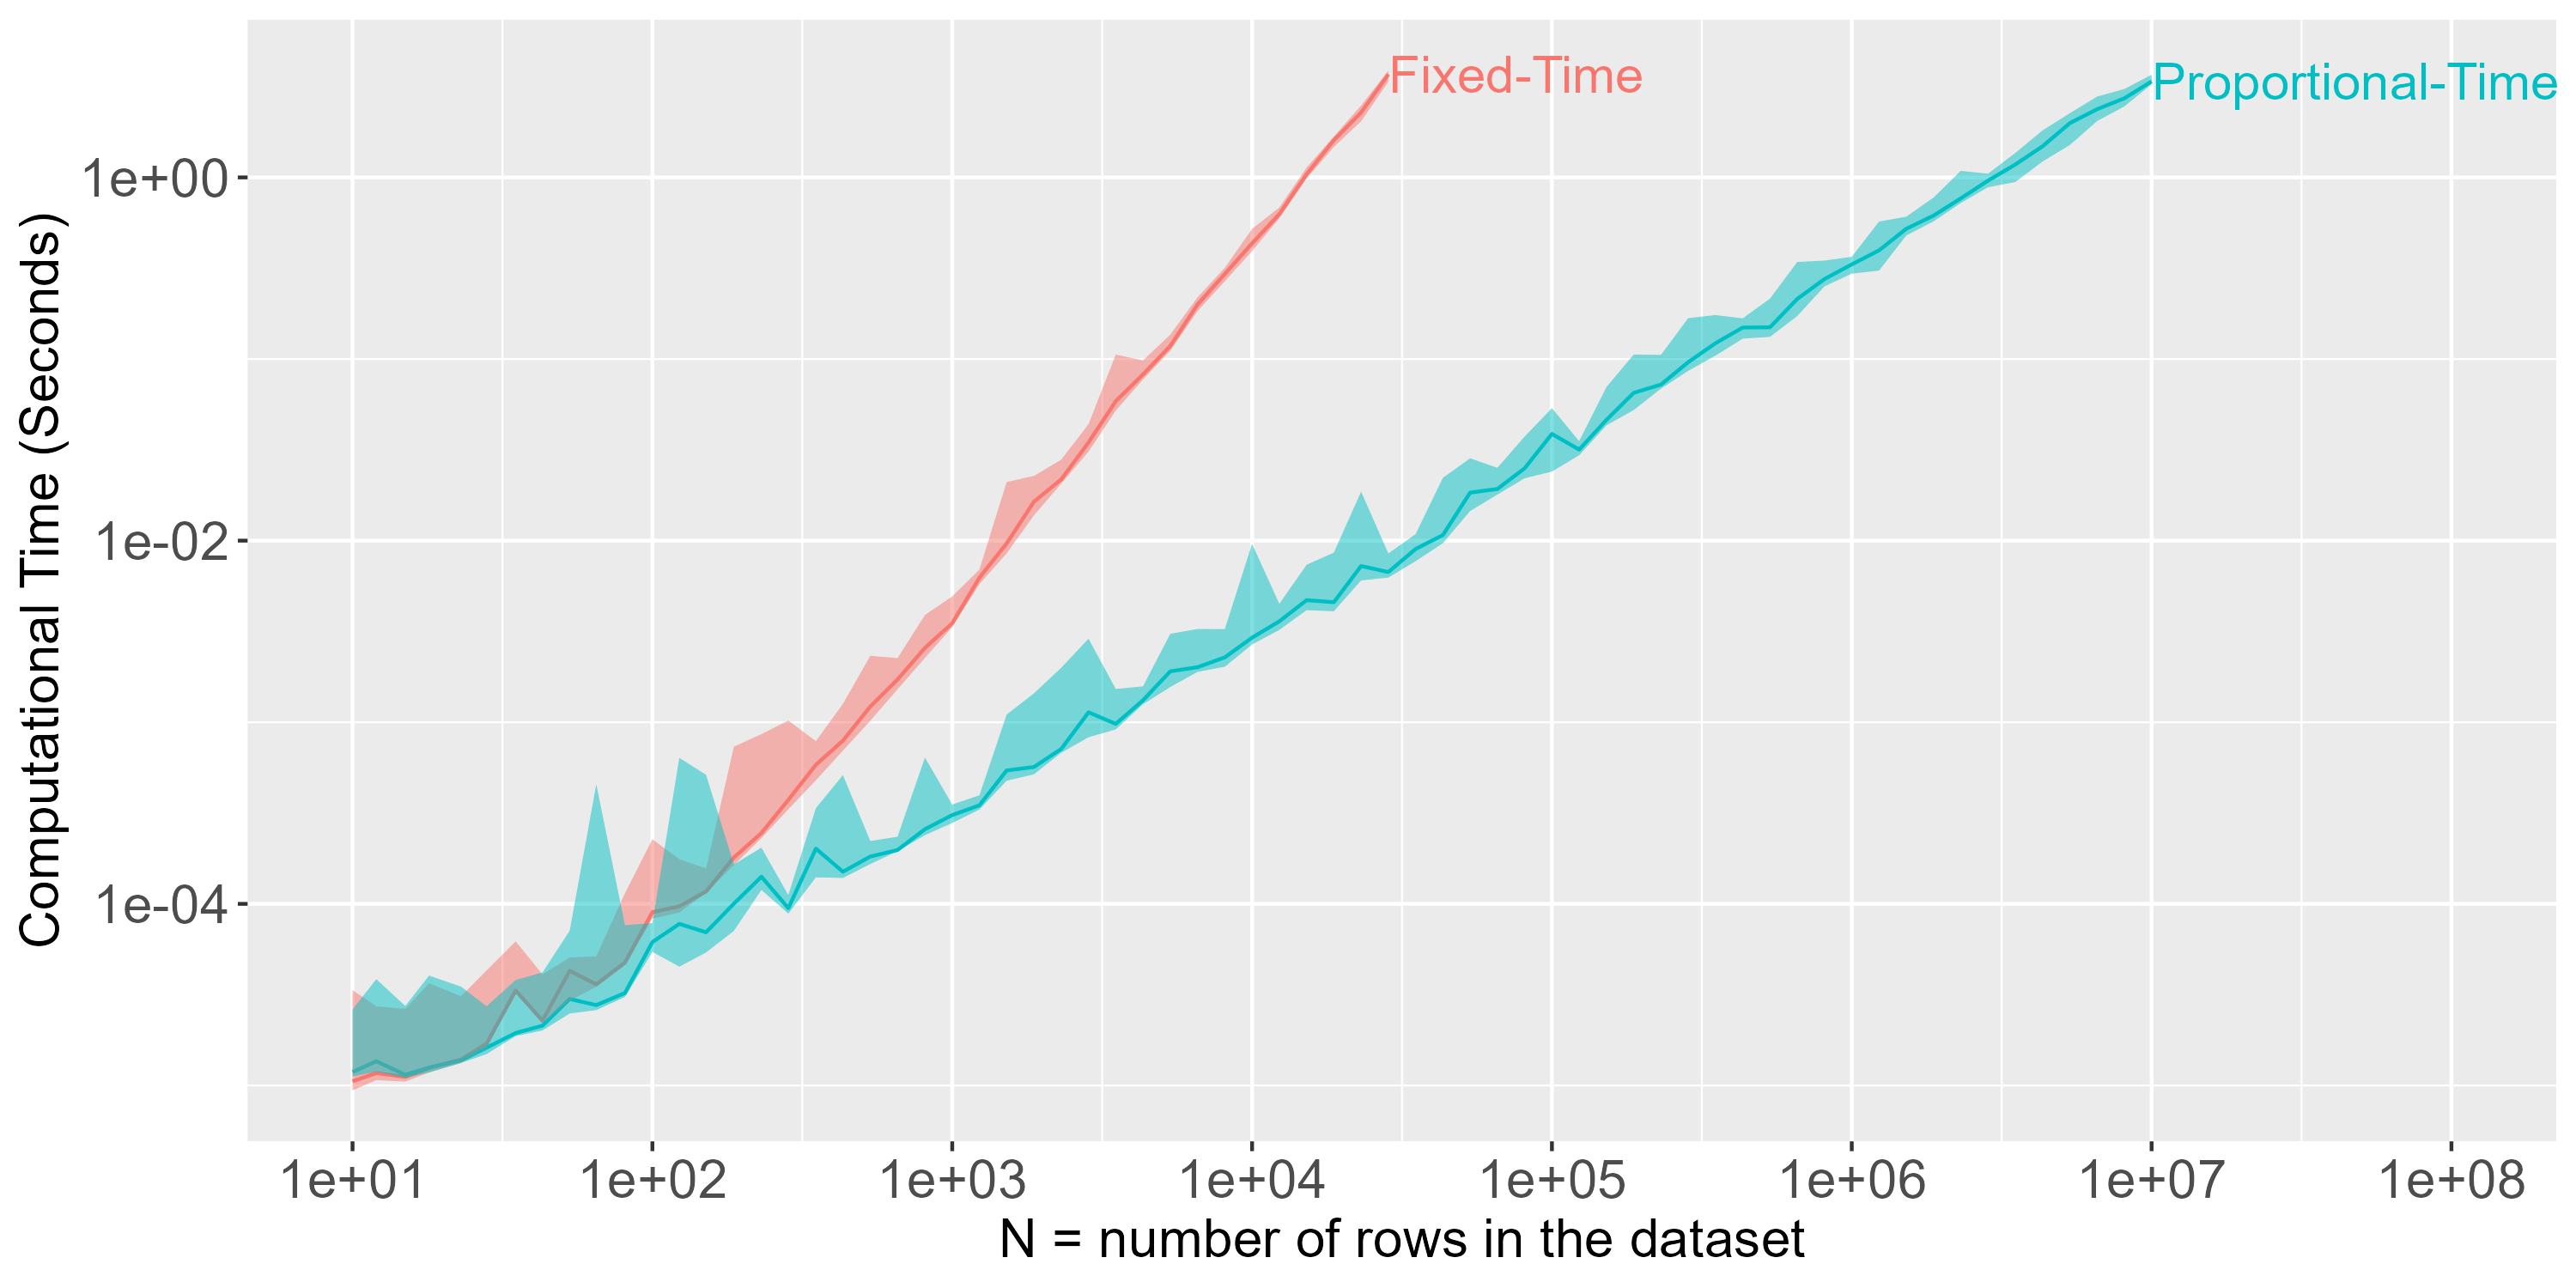
\includegraphics[width=0.8\linewidth]{figures/best.list.R.png}
    \caption{showing the best fit asymptotic time complexity for each linear and constant timings}
    \label{fig:label1}
\end{figure}

\noindent The goal of creating this figure is to understand how computational time scales with increasing dataset size for two different scenarios: one with fixed time complexity and another with time proportional to some function of N. As expected, the computational time for the fixed-time scenario remains relatively constant, while the proportional-time scenario shows a more rapid increase as the dataset size grows. The figure confirms this expectation, with both computational times increasing as N increases, but the proportional-time line showing a steeper increase. For smaller values of N, both scenarios have similar computational times, but they diverge significantly for larger values of N. This figure reveals that while both fixed-time and proportional-time computations take longer with larger datasets, proportional-time computation becomes significantly more time-consuming as dataset size grows very large, providing crucial insight for choosing between different algorithms on their expected performance with large amounts of data.\\


\subsection{Comparative Benchmarking}

\noindent Comparative benchmarking is the process of comparing the performance of different algorithms or approaches for benchmarking. It allows us to assess packages performance against different packages and algorithms by measuring execution time and memory usage.\\

\noindent atime offers comparative benchmarking technique to evaluate packages, providing insights into performance efficiency. By conducting a comparative benchmark these tests, we ensure package remains a high-performance tool for data analysis, delivering reliable results for end-users\\

\subsubsection{Comparing R packages performing similar Task.}
\noindent When working with data in R, we all want to know which tools are the most efficient. That is why we're putting some of the most popular R packages to the test. 
In this section, we would demonstrate how to use atime for comparative benchmarking for three R functions that perform the same task. We will demonstrate the advantages of using atime for comparative benchmarking over other R packages. The major advantage is it allows us to alternate the expressions over different N sizes. Another advantage is it gives you a more appropriate and easy interpretation of your results visually.\\

\noindent For example, consider the following simple example of comparatively benchmarking three functions from the R packages \code{data.table}, \code{utils} and \code{readr} for reading a CSV file. Our goal is to provide an idea as to which packages are the fastest and most memory-efficient, so people can choose the best ones for their data analysis needs.\\

\begin{lstlisting}[language=R]
> n.rows <- 100
> seconds.limit <- 5
> atime.read.vary.cols <- atime::atime(
+   N = as.integer(10^seq(2, 6, by = 0.5)),
+   setup = {
+     set.seed(1)
+     input.vec <- rnorm(n.rows * N)
+     input.mat <- matrix(input.vec, n.rows, N)
+     input.df <- data.frame(input.mat)
+     input.csv <- tempfile()
+     fwrite(input.df, input.csv)
+   },
+   seconds.limit = seconds.limit,
+   "data.table::fread" = {
+     data.table::fread(input.csv, showProgress = FALSE)
+   },
+   "readr::read_csv\n(lazy=TRUE)" = {
+     readr::read_csv(input.csv, progress = FALSE, show_col_types = FALSE, lazy = TRUE)
+   },
+   "utils::read.csv" = utils::read.csv(input.csv)
+ )
\end{lstlisting}

The code above uses the \code{atime()} package to measure and compare the performance (time and memory usage) of different R functions for reading CSV files as the size of the input data increases. Here's a step-by-step breakdown:

\begin{itemize}
    \item \textbf{Parameters:}
    \begin{itemize}
        \item \texttt{n.rows} is set to 100, representing the number of rows in the input data.
        \item \texttt{seconds.limit} is set to 5, the maximum time allowed for each operation.
    \end{itemize}

    \item \textbf{Defining the \texttt{atime.read.vary.cols} Object:}
    \begin{itemize}
        \item The \texttt{atime::atime} function is used to benchmark different reading functions.
        \item \texttt{N} is a sequence of increasing sizes of data (\(10^2\) to \(10^6\), incremented by 0.5 powers of 10).
    \end{itemize}

    \item \textbf{Setup:}
    \begin{itemize}
        \item A random seed is set for reproducibility.
        \item A vector of random numbers is generated and reshaped into a matrix with \texttt{n.rows} rows and \texttt{N} columns.
        \item This matrix is converted into a data frame.
        \item The data frame is written to a temporary CSV file.
    \end{itemize}

    \item \textbf{Benchmarking:}
    \begin{itemize}
        \item Three different functions are benchmarked for reading the CSV file:
        \begin{itemize}
            \item \texttt{data.table::fread}: Reads the CSV using the \texttt{data.table} package.
            \item \texttt{readr::read\_csv}: Reads the CSV using the \texttt{readr} package with lazy evaluation.
            \item \texttt{utils::read.csv}: Reads the CSV using the base R function.
        \end{itemize}
    \end{itemize}
\end{itemize}

\begin{verbatim}
List of 3
 $ unit.col.vec : Named chr [1:2] "kilobytes" "median"
  ..- attr(*, "names")= chr [1:2] "" "seconds"
 $ seconds.limit: num 5
 $ measurements :Classes ‘data.table’ and 'data.frame':	19 obs. of  17 variables.
\end{verbatim}

\begin{itemize}
    \item \textbf{unit.col.vec:} Named character vector of length 2, with values "kilobytes" and "median".
    \begin{itemize}
        \item The attributes contain names, which are "" and "seconds".
    \end{itemize}

    \item \textbf{seconds.limit:} Numeric value of 5, indicating the maximum allowed time for each operation.

    \item \textbf{measurements:} A \texttt{data.table} and \texttt{data.frame} with 19 observations and 17 variables.
\end{itemize}

\noindent The output is a list of three elements, including \texttt{unit.col.vec}, \texttt{seconds.limit}, and \texttt{measurements}, of which each measurement is of class \texttt{data.table} and \texttt{data.frame}. The \texttt{unit.col.vec} is a named character vector with units ("kilobytes" and "median"), and \texttt{seconds.limit} is a numeric value set to 5. The \texttt{measurements} contain 19 observations and 17 variables. These data can be used to create the desired plot with \texttt{ggplot2}.


\begin{figure}[H]
    \centering
    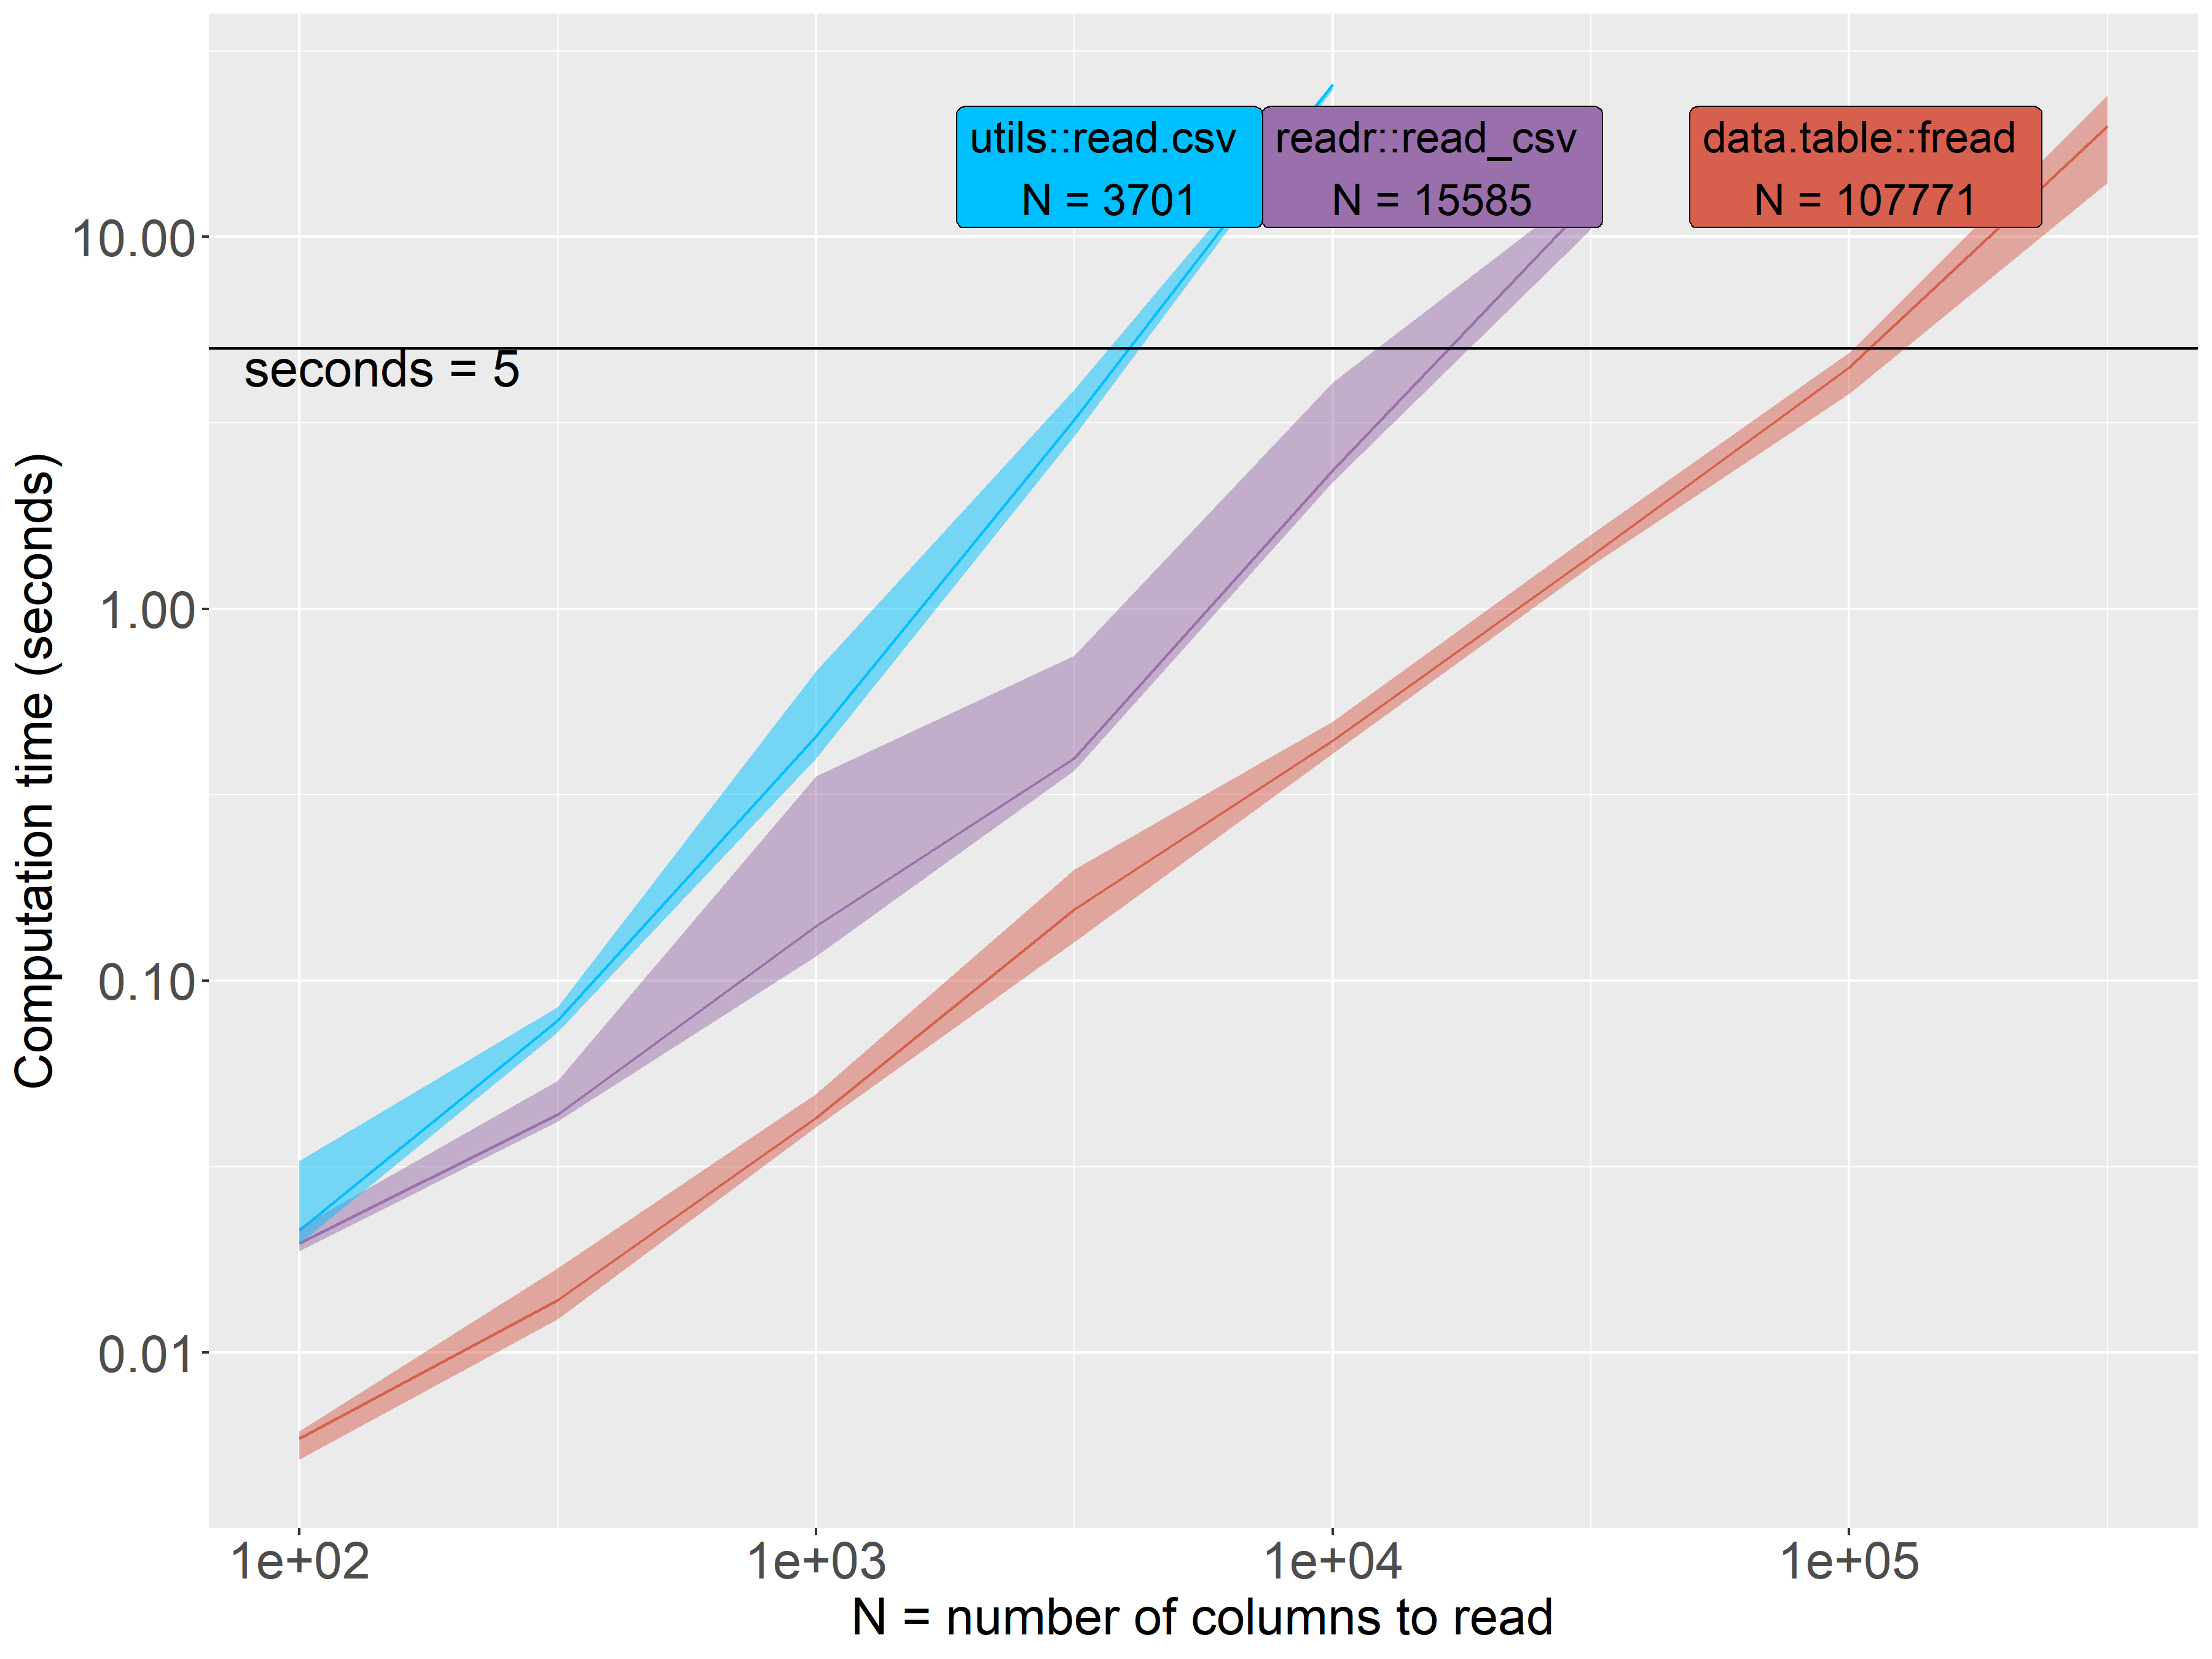
\includegraphics[width=0.7\linewidth]{figures/gg.read.3.png}
    \caption{Comparing different functions for reading a csv file}
    \label{fig:label2}
\end{figure}

\noindent Figure 2 is comparing the performance of three different methods for reading data into R \texttt{utils::read\_csv}, \texttt{readr::read\_csv}, and \texttt{data.table::fread} as the number of columns increases. As expected, the computation time for each method increases with the number of columns, but at different rates, revealing which method is more efficient for larger datasets. The figure shows that \texttt{data.table::fread} is consistently faster than the others across all column sizes, with \texttt{utils::read\_csv} and \texttt{readr::read\_csv} taking longer as the number of columns grows. The N-values (3701, 15855, and 10771) represent the sample size for each method, providing context for the variability and confidence intervals shown in the graph. Overall, this figure reveals that \texttt{data.table::fread} is the most efficient method, especially for larger datasets, providing crucial insight for choosing the best method for reading large data files in R.\\


\subsection{Performance Testing}
The \texttt{atime} package provies a function named \texttt{atime\_pkg()} which enables users to integrate asymptotic timing and memory analysis into continuous integration and deployment workflows. 
This can help ensure that new changes to R packages do not introduce performance regressions. When performing these performance tests, we use \texttt{atime::atime\_versions}.
Performance testing can be done on any R package written with \texttt{Rcpp}.\\

\noindent we will discuss how to use \texttt{atime::atime\_versions} to create performance testing for the \texttt{data.table} package in R.
\texttt{data.table} is a powerful extension of R's data.frame, designed to handle large datasets with exceptional efficiency. Its concise and expressive syntax enables users to perform complex data manipulations with ease, making it an ideal tool for data analysis. The development team behind \texttt{data.table} is dedicated to continuously optimize its performance, ensuring swift execution of tasks like filtering, grouping, aggregating, and joining data.
\vspace{0.1in}
To guarantee high-performance standards, \texttt{data.table} employs a robust performance testing framework. This framework measures the actual execution time of specific operations, enabling accurate comparisons between different package versions. 
Our \texttt{atime}-based performance tests aim to assess packages by benchmarking performance and gathering information on memory and time usage. 
\vspace{0.1in}
By conducting these tests, we gain valuable insights into a package's performance efficiency, ensuring the delivery of a reliable package to users.
\vspace{0.1in}

\noindent Approach

\begin{itemize}
    
\item \textit{To begin} conduct the atime test for the different code branches (before regression, regression, fix regression) to identify potential performance issues. 
\vspace{0.1in}

\noindent Note: Set up the necessary environment and dependencies, ensuring that the data.table and atime packages are installed and loaded.
\vspace{0.1in}

\item \textit{Generate} a plot to showcase the fixes made in the data.table package using the atime package.

\vspace{0.1in}
\item \textit{utilize} the atime::atime\_versions function to track the fixes across different versions.
\vspace{0.1in}

\item \textit{pass} the following named arguments to atime::atime\_versions: N, setup, expr, and the different code branches. More documentation of the atime package can be found [here](https://github.com/tdhock/atime). 
\vspace{0.1in}

\item \textit{use} the plot function to visually present the execution times of the expression evaluated across different versions of the data.table package

\end{itemize}

\textbf{What are the Performance Tests?}

Our \code{atime()} performance tests aim to assess the \texttt{data.table} repository by benchmarking its performance and gathering information on memory and time usage. By conducting these tests, we can gain insights into the package’s performance efficiency.

When using \texttt{atime\_versions}, there are six main arguments:

\begin{enumerate}
    \item \textbf{pkg.path:} This argument specifies the location on your system where you have stored a git clone of the \texttt{data.table} package.
       
    \item \textbf{expr:} This section contains the expression that represents the operation being benchmarked. It uses the \texttt{data.table::[.data.table]} syntax to perform the operation on the dataset. In the given syntax \texttt{data.table::[.data.table]}, the first part \texttt{data.table::} installs and loads different versions of the \texttt{data.table} package based on the specified commit IDs. Hence, \texttt{data.table::} will be translated to \texttt{data.table.SHA1::} for some version hash SHA1. Following that, the expression specified within \texttt{[.data.table]} is executed on each installed version. This process is repeated for all the specified commit IDs in the code.
 
    \item \textbf{... :} This section specifies the different versions of the \texttt{data.table} packages that will be tested. It includes three versions: ``Before,'' ``Regression,'' and ``Fixed.'' Each version is associated with a specific commit ID.
\end{enumerate}

We run the full performance regression:

\begin{enumerate}
    \item Before the performance regression is made (Before)
    \item When the performance regression is first submitted (Regression/Slow)
    \item Pull Request (PR) which fixes the performance regression (Fixed/Fast)
\end{enumerate}


\noindent Performance Test case with two code branches: fast and slow:\\

\begin{lstlisting}[language=R]
> atime.list <- atime::atime_versions(
+   pkg.path = "~/data.table",
+   pkg.edit.fun = pkg.edit.fun,
+   N = 10^seq(1, 7, by = 0.25),
+   setup = { 
+     DT <- replicate(N, 1, simplify = FALSE)
+   },
+   expr = data.table:::setDT(DT),
+   "Slow" = "c4a2085e35689a108d67dacb2f8261e4964d7e12",
+   "Fast" = "1872f473b20fdcddc5c1b35d79fe9229cd9a1d15"
+ )
\end{lstlisting}

\noindent The code above benchmarks the performance of different versions of the data.table package by measuring the computational time for a specific setDT operation on a data.table with varying numbers of rows. It helps in understanding the impact of the regression and the effectiveness of the fix. \\


\begin{figure}[H]
    \centering
    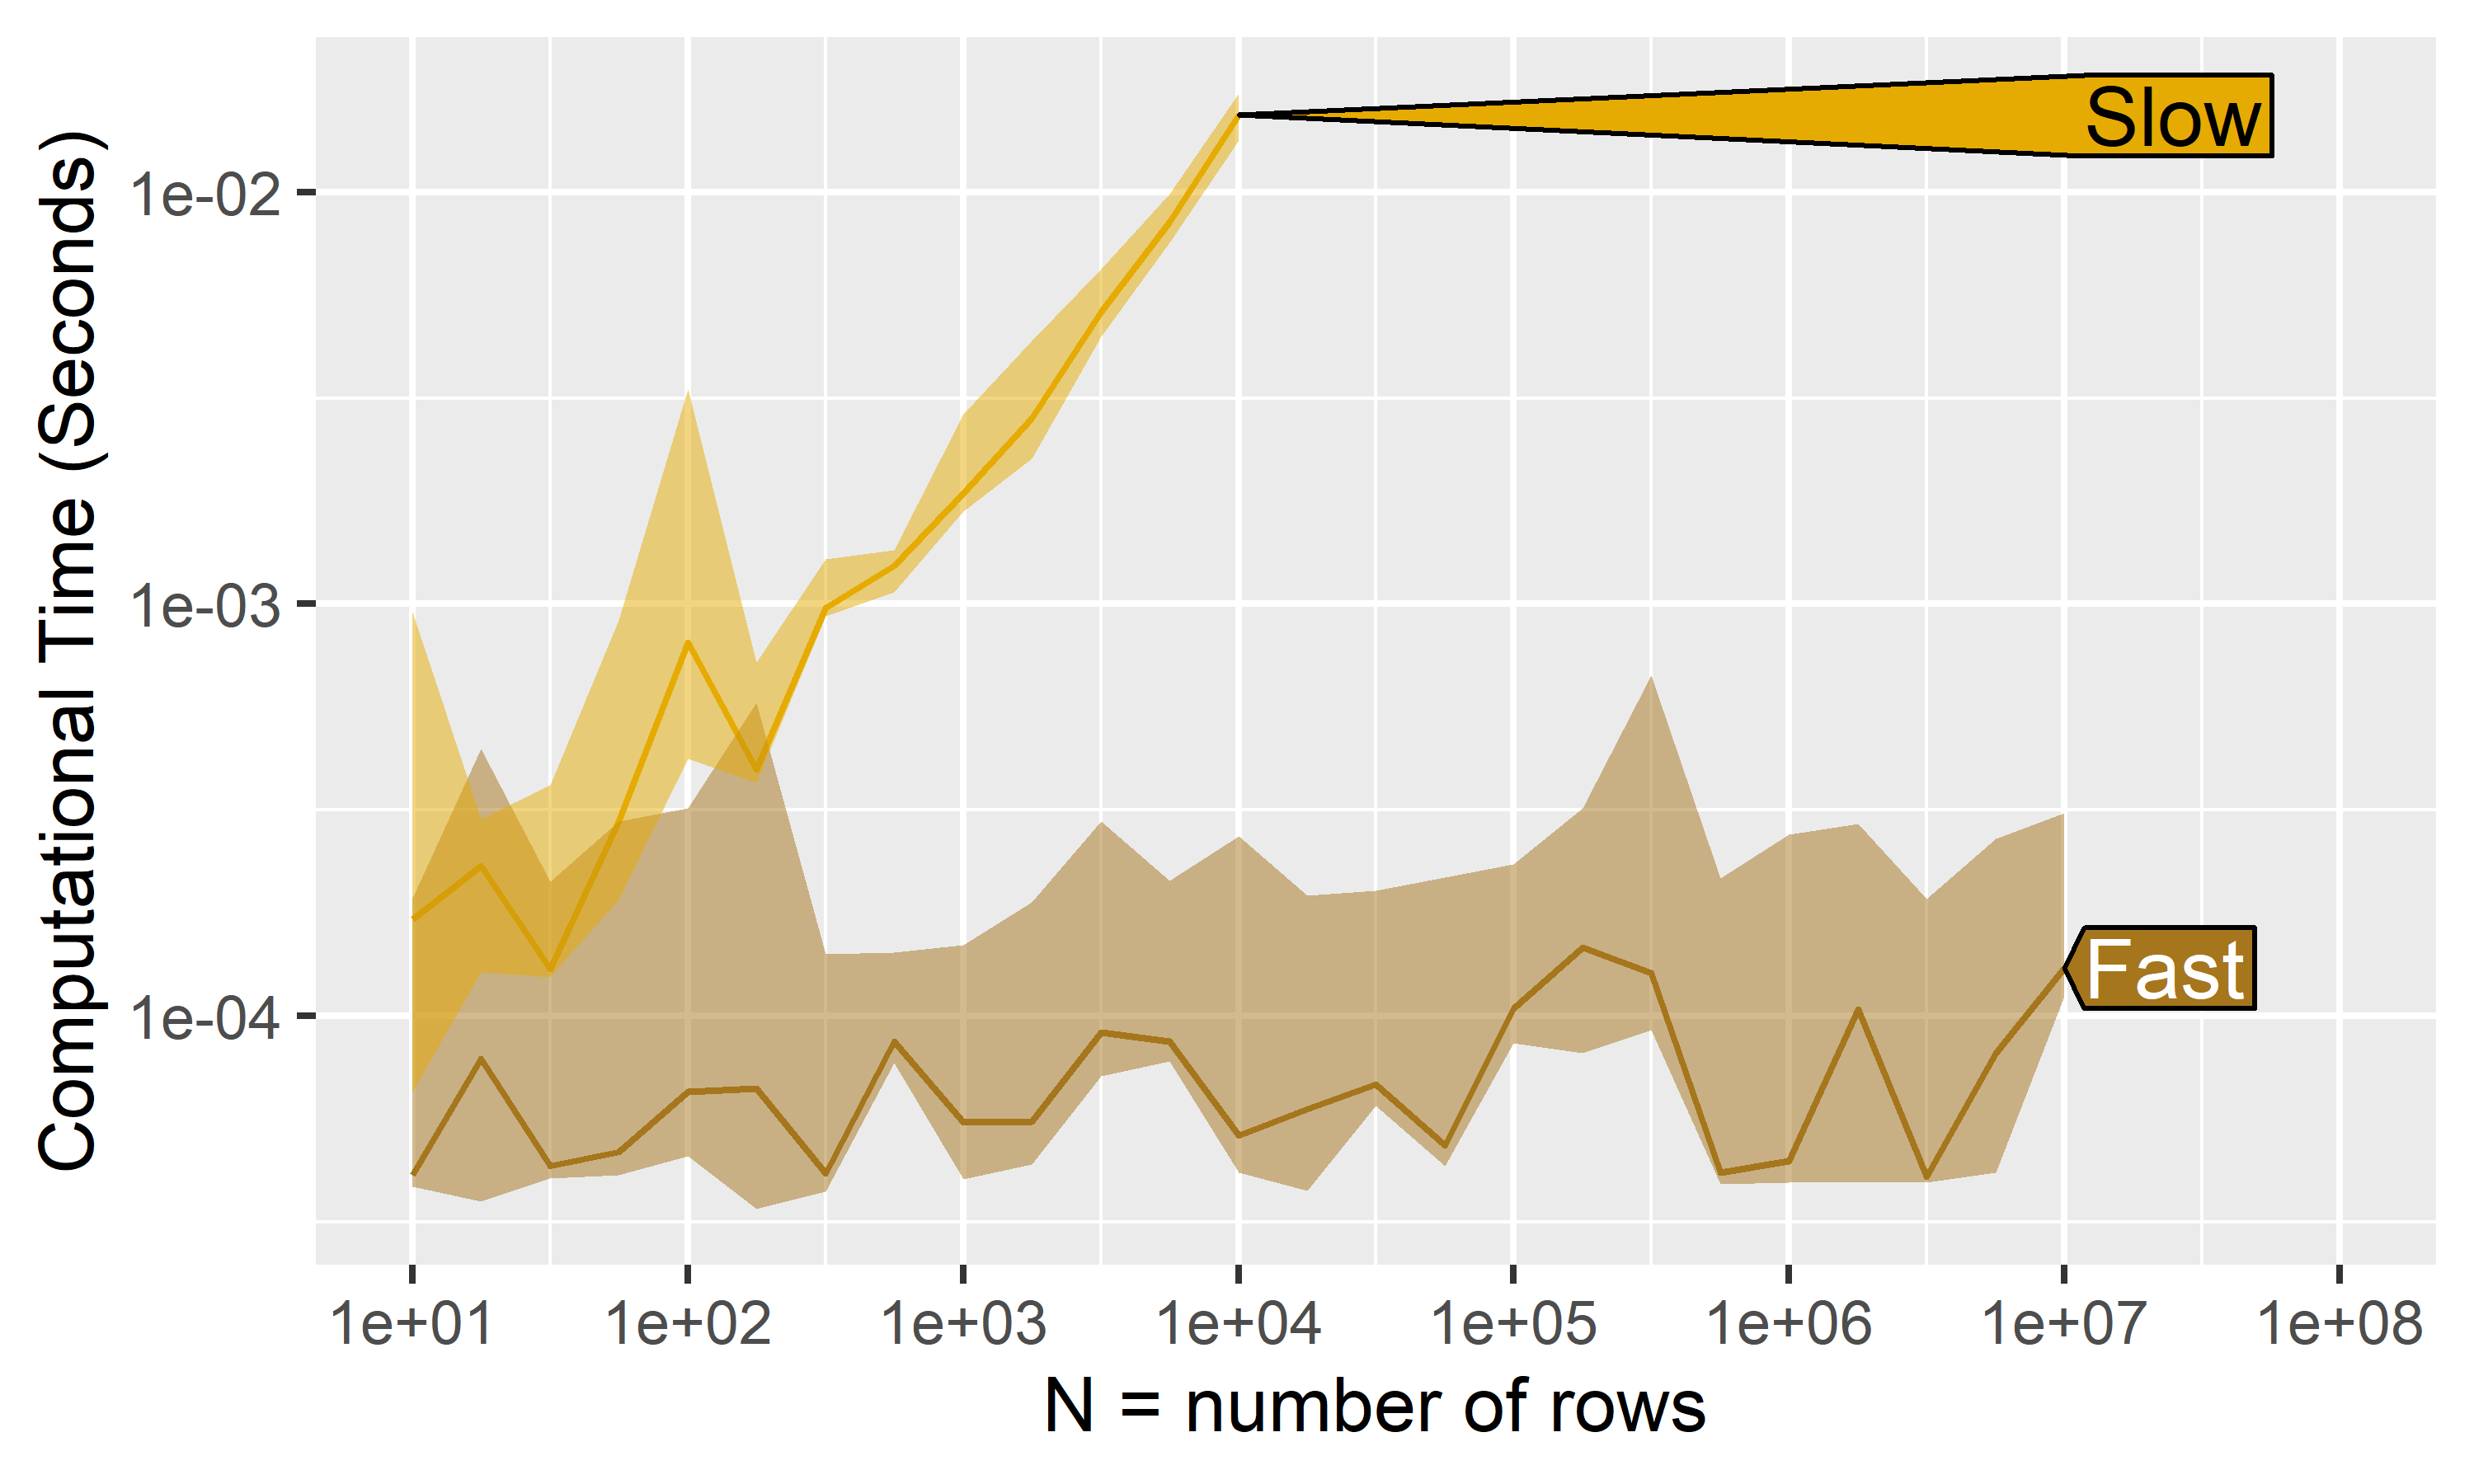
\includegraphics[width=0.6\linewidth]{figures/atime.list.5427.png}
    \caption{Performance Test case with two code branches: fast and slow}
    \label{fig:label3}
\end{figure}

\noindent We created a performance test from the pull request reported on the data.table repository with the goal of comparing the computational time of two versions of data.table package, one with a regression causing slowness ("Slow") and a newer version ("Fast") released to mitigate the regression and improve performance. As expected, the "Slow" version exhibits higher computational times as the number of rows increases, while the "Fast" version maintains lower computational times, demonstrating improved performance and efficiency. The figure shows that for smaller datasets, both versions have similar computational times, but as the number of rows grows, the "Slow" version becomes significantly slower, whereas the "Fast" version maintains a lower computational time. This comparison clearly shows that the new "Fast" version successfully mitigates the regression and enhances performance. The output captures the computational time for each version of the data.table package (Fast and Slow) across different dataset sizes, providing a comprehensive understanding of the impact of the regression and the effectiveness of the new version.\\

\noindent Performance Test case with three code branches: Regression, Fixed and Before: \\

\begin{lstlisting}[language=R]
> atime.list <- atime::atime_versions(
+   pkg.path = "~/data.table",
+   pkg.edit.fun = pkg.edit.fun,
+   N = 10^seq(1, 7, by = 0.25),
+   setup = { 
+     set.seed(108)
+     d <- data.table(
+       id3 = sample(c(seq.int(N * 0.9), sample(N * 0.9, N * 0.1, TRUE))),
+       v1 = sample(5L, N, TRUE),
+       v2 = sample(5L, N, TRUE))
+   },
+   expr = data.table:::`[.data.table`(d, , (max(v1) - min(v2)), by = id3),
+   "Before" = "793f8545c363d222de18ac892bc7abb80154e724",
+   "Regression" = "c152ced0e5799acee1589910c69c1a2c6586b95d",
+   "Fixed" = "f750448a2efcd258b3aba57136ee6a95ce56b302"
+ )
\end{lstlisting}

\noindent This code above is almost as the first simple, except it has three code branches Before, Regression and Fixed. it benchmarks the performance of different versions of the data.table package by measuring the computational time for a specific operation on a data.table with varying numbers of rows.
The output as mentioned previously will capture the computational time for each version of the data.table package (Before, Regression, and Fixed) across different dataset sizes. It will compare the performance of these versions, highlighting the impact of the regression and the effectiveness of the fix. \\


    \begin{verbatim}
    data.table.793f8545c363d222de18ac892bc7abb80154e724::`[.data.table`(d, , (max(v1) - min(v2)), by = id3)  
    \end{verbatim}
    
\vspace{0.1in}
\noindent In this code, the expression \texttt{[.data.table]} is executed on the \texttt{d} dataset using the specified commit IDs (793f8545c363d222de18ac892bc7abb80154e724) of the \texttt{data.table} package. The expression calculates the difference between the maximum value of \texttt{v1} and the minimum value of \texttt{v2}, and is grouped by \texttt{id3}. This process is repeated for all commit IDs in the code to compare the performance of different versions of the \texttt{data.table} package.\\

\begin{figure}[H]
    \centering
    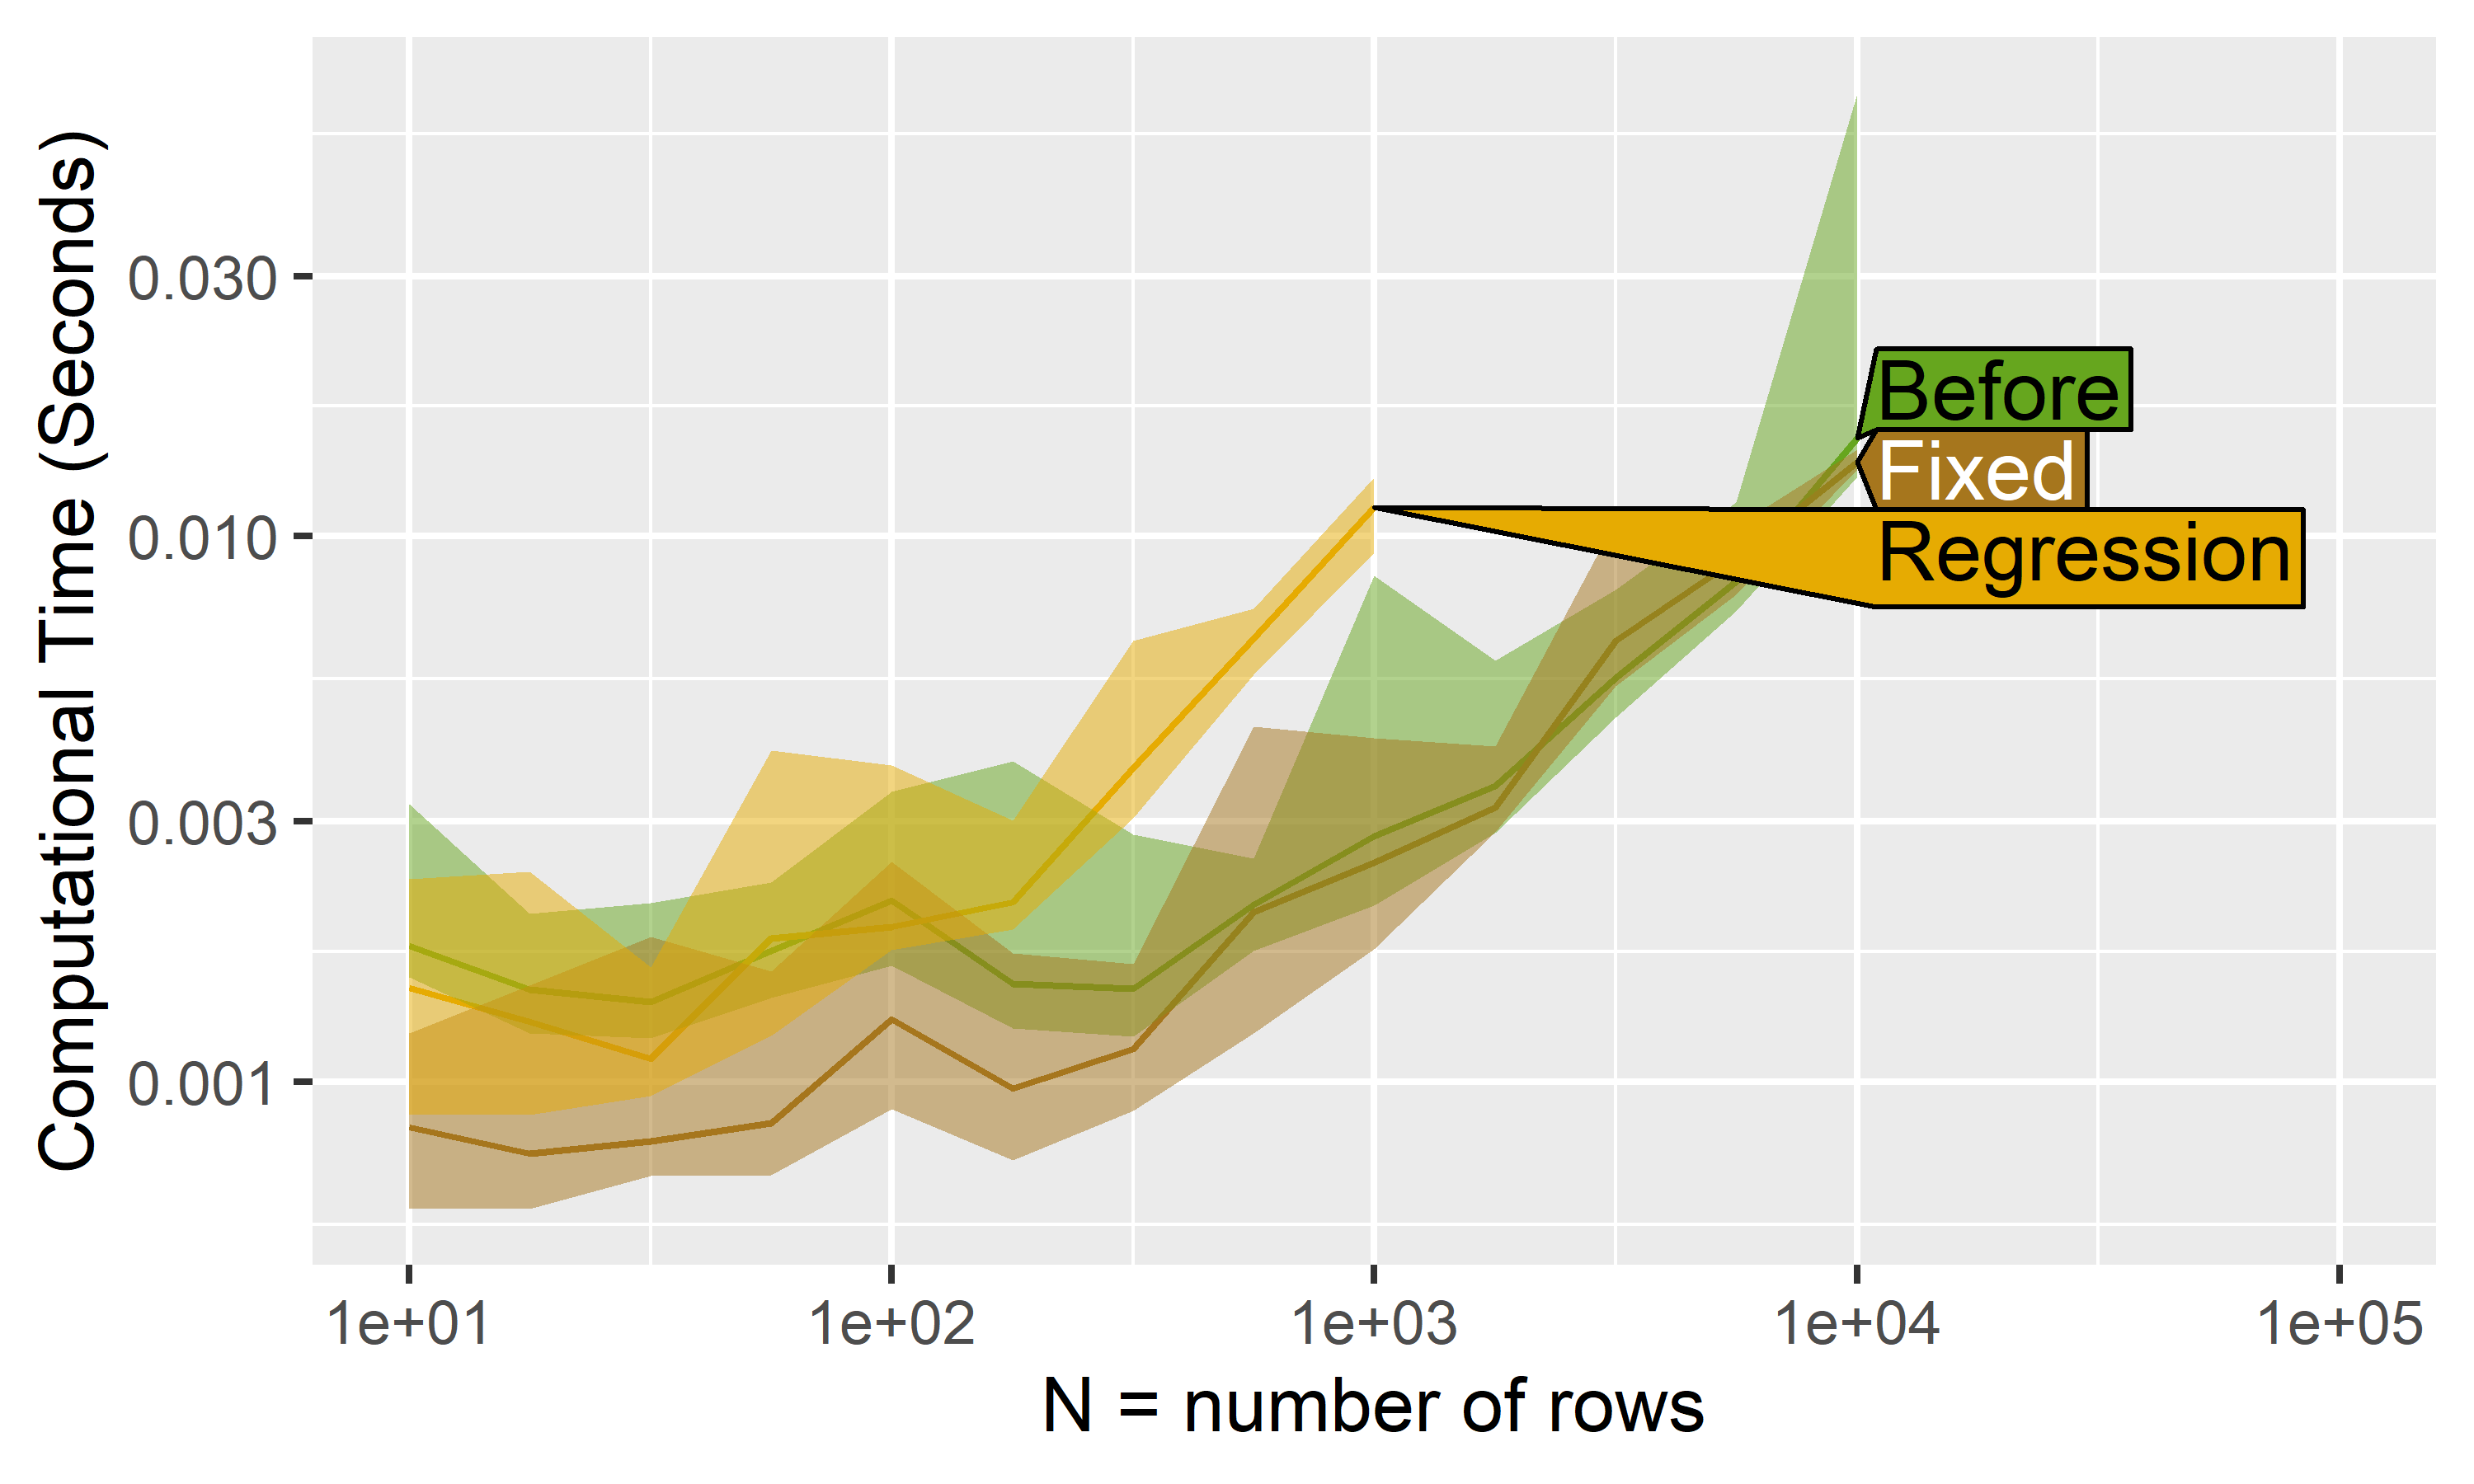
\includegraphics[width=0.7\linewidth]{figures/atime.list.4200.png}
    \caption{Performance Test case with three code branches: Regression, Fixed and Before}
    \label{fig:label4}
\end{figure}

\noindent Again we explore the data.table repository, to find pull requests relating to three code branches, to show another performance test. The figure compares the computational time of three package versions - Before, Regression, and Fixed (after a regression was improved or fixed) to understand the impact of the regression and the effectiveness of the fix. As expected, computational time increases during the Regression phase and decreases after the fix, either returning to or improving upon the pre-regression time (Before). The figure shows three distinct regions: a stable Before region, a slower Regression region, and a faster Fixed region, indicating the regression's significant impact and the fix's effectiveness in mitigating it. Overall, the regression substantially increased computational time, but the fix successfully restored or even improved performance, making the package more efficient.\\


\section{Performance Testing with GitHub Actions CI}
\section{Section by Anirban Chetia}

A GitHub Action was created by Anirban to facilitate performance testing of the incoming changes that are introduced via Pull Requests (PRs) to the GitHub repositories of R packages. The primary motivation behind this was to help ensure that \code{data.table}, a popular R package, maintains its code efficiency or high-performance standards (core values of the project) as PRs keep coming and getting integrated frequently into the codebase, meaning they need to be monitored for performance regressions, and an automatic way to do that would be ideal.
\newline
\newline
The key features of this GitHub Action include:
\begin{itemize}
    \item \textbf{Predefined flexible tests} 
    \newline
    The action runs test cases (utilizing the \code{atime} package) from the setup defined in \code{.ci/atime/tests.R} (can be customized) on different versions of \code{data.table} or the R package being tested. These tests are either based on documented historical regressions or performance improvements.
    \item \textbf{Automated commenting}
    \newline
    Using \code{cml}, the action publishes results in a GitHub-bot authored comment on the pull request thread. The comment gets updated time and again on new pushes to avoid cluttering (ensuring only one comment exists per PR, updated with the latest information concisely). 
    \item \textbf{Diagnostic visualization}
    \newline
    A plot is uploaded within the comment which comprises of subplots for each test case, showing the time and memory trends across different \code{data.table} versions.
    \item \textbf{Timing information}
    \newline
    The time taken (in seconds) for setup and test execution is supplied within the comment as well.
    \item \textbf{Links}
    \newline
    A download link for the artifact containing all the \code{atime}-generated results is provisioned, apart from the GitHub link to the commit SHA that generated the latest plot results.

    \item \textbf{Versioning}
    \newline
    The action computes the tests on different \code{data.table} versions that can be visually compared on the resultant plot. These include various labels, as described in the table below:
    \begin{table}[H]
        \centering
            \caption{Version labels}
        \begin{tabular}    
        {|m{1.9cm}|m{10.8cm}|}
  \hline
  Label name & R package version description \\
  \hline
  base   & PR target  \\
  \hline
  HEAD   & PR source  \\
  \hline  
  Merge-base   & The common ancestor between base and HEAD \\
  \hline
  CRAN   & Latest version on the CRAN platform  \\
  \hline
  Before   & Pre-regression commit  \\
  \hline
  Regression   & The commit (or if the source is unknown or distributed, the range of commits) which is responsible for the performance degradation  \\
  \hline  
  Fixed   & Commit where the performance has been restored or improved beyond the point of regression  \\
  \hline
    \end{tabular}
\end{table}
\end{itemize}

The action is not constrained to be OS-specific and there is only one single job or set of steps that execute on the same runner.
\newline
\newline
There are ample examples of this in action within the official \code{data.table} GitHub repository's 'Pull requests' section (actively running as new PRs involving code changes emerge). The figure below is taken from one of those recent (at the time of writing) runs.

\begin{figure}[H]
    \centering
    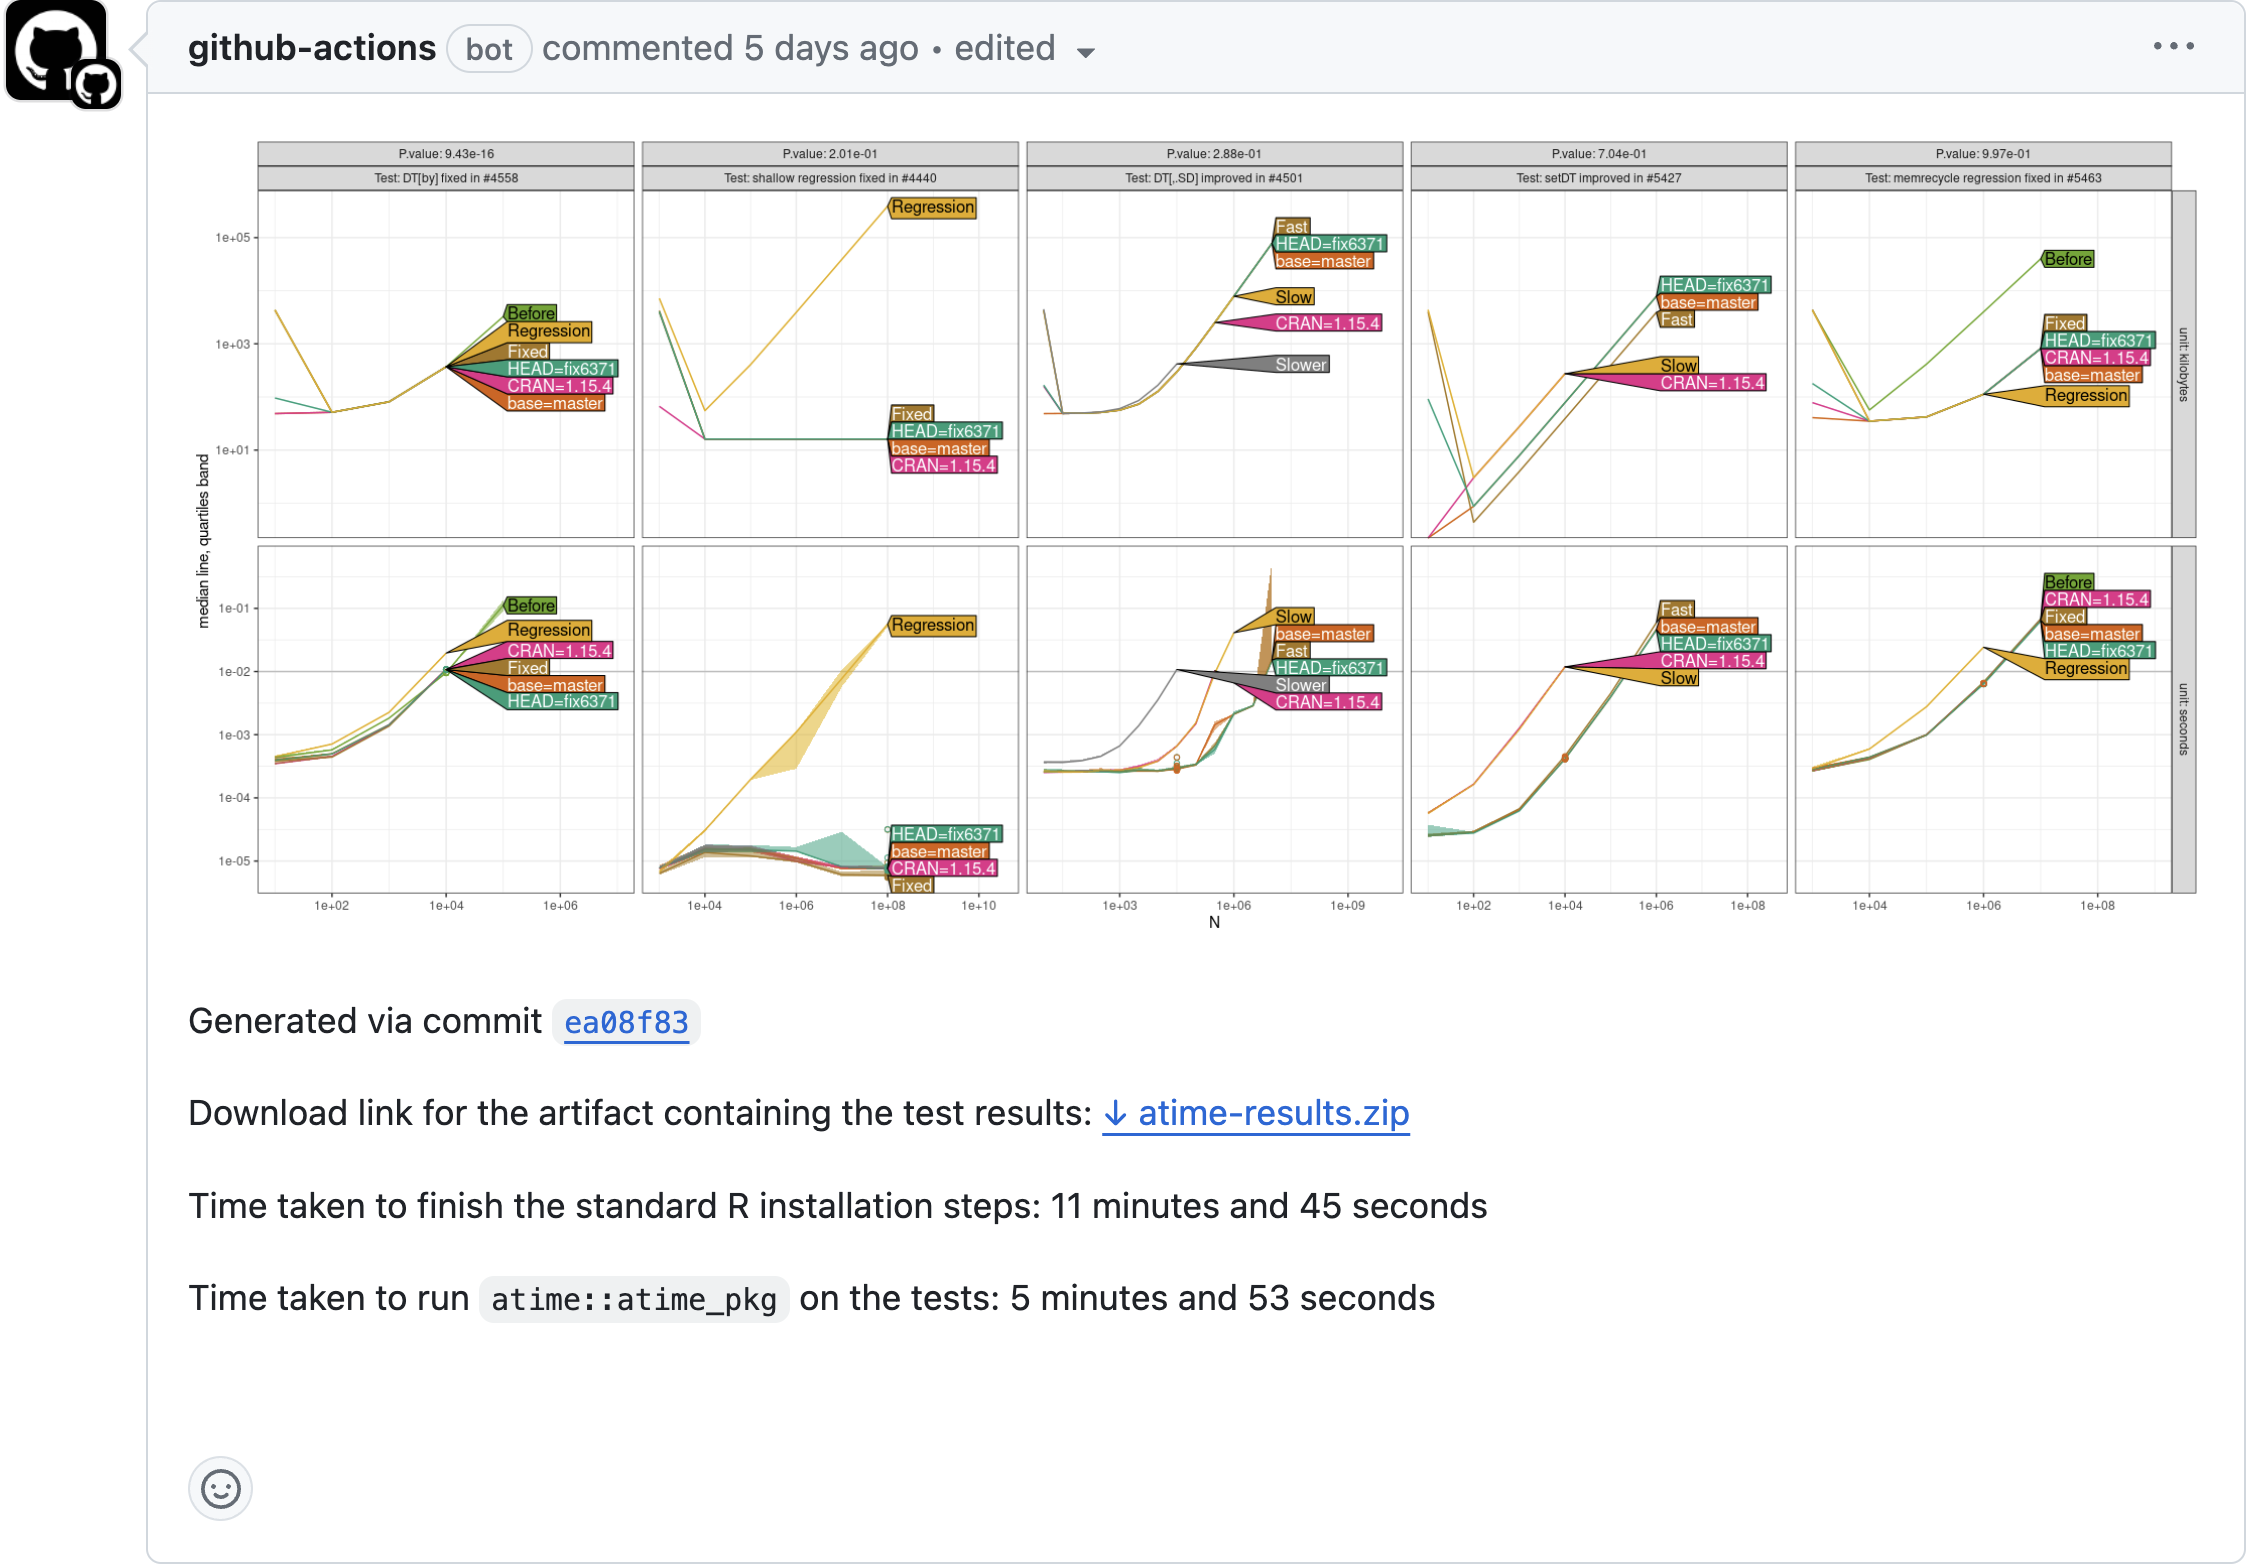
\includegraphics[width=1.0\linewidth]{figures/GHA2.png}
    \caption{Test cases running for every code changing PR via the GitHub Action that Anirban created}
    \label{fig:label5}
\end{figure}


\section{Discussion and conclusions}

In this paper, we described the \code{atime()} package and its new functions for comparative benchmarking, performance testing, and continuous performance testing through GitHub Actions. We demonstrated how the syntax of \code{atime()} makes it easy to define and use its functions for various types of performance evaluations.

Through several examples, we showcased the versatility of \code{atime()} in performing different comparisons and performance tests. Our detailed comparison with other benchmarking packages and functions highlighted the advantages of \code{atime()}, including its ability to specify a range of data sizes and facilitate result visualization.

We also demonstrated \code{atime()}'s capacity to handle both constant and linear asymptotic time complexity, making it a valuable tool for performance analysis. Furthermore, we discussed the design choice to keep separate functions for comparative benchmarking and performance testing, allowing for more specific and informative documentation, examples, and error messages.

\code{atime()} features two distinct functions for benchmarking: 
\begin{itemize}
 

    \item\texttt{atime::atime} for comparative benchmarking \item\texttt{atime::atime\_versions} for performance testing and continuous performance testing. 

\end{itemize}

While it is possible to merge these functions into a single function, we intentionally maintain their separation to provide detailed documentation, relevant examples, and informative error messages, ultimately enhancing the user experience.

Overall, our work introduces \code{atime()} as a comprehensive and user-friendly package for performance testing and comparative benchmarking, offering a range of functions and features that make it an essential tool for developers and researchers. By providing a detailed understanding of \code{atime()}'s capabilities and advantages, we hope to encourage its adoption and contribute to the development of more efficient and scalable software solutions.






\bibliography{DorisAmoakohene}

